% For help on this document class, see:
% https://ftp.tu-chemnitz.de/pub/tex/macros/latex/contrib/acmart/acmart.pdf
\documentclass[acmtog, language=english, nonacm]{acmart}

\usepackage{cleveref}
\usepackage[T1]{fontenc}
\usepackage{fullpage}
\usepackage[utf8]{inputenc}
\usepackage{siunitx}
\usepackage{tikz}
\usepackage[european]{circuitikz}
\usepackage{titlesec}

\setlength{\headheight}{11.0pt}
\setlength{\parindent}{0pt}

\titleformat{\section}{\normalsize\bfseries}{\thesection}{1em}{}
\titleformat{\subsection}{\normalsize\bfseries}{\thesubsection}{1em}{}
\titleformat{\subsubsection}{\normalsize\bfseries}{\thesubsubsection}{1em}{}

\title{Software Project Report: \textsc{Lattice Watering}}
\author{Valentin Pickel}
\email{valentinpickel@gmx.de}
\author{Jonas Heinemann}
\author{Christian Müller}
\author{Kaan Dönmez}
\affiliation{%
    \department[0]{Institute for Computer Science}%
    \institution{Freie Universität Berlin}%
    \city{Berlin}%
    \country{Germany}}


\begin{document}
    \maketitle

    \section{Introduction}

    We may start from scratch by reminiscing the the first meeting of all course participants on April 4th. This software project course should dive into the ecosystem internet. To do so, a rough split was set between the worlds of the \emph{Internet of Things} (IoT), which deals with low power devices in large networks plagued with packet loss, and the conventional internet and its vastly more potent desktop computers and servers. Especially, us students should become aware of design decisions with respect to the communication solutions that our software should utilize. The project \emph{Lattice Watering} eyes out the first of both worlds.

    \subsection{Idea Outline}

    After suggesting the building an IoT application for watering plants automatically on May 2nd, the software project \emph{Lattice Watering} and its group formed on the 9th of May, comprising of the aforementioned members. The term \emph{Lattice} is a reference to the studies of crystal/grid-like molecular structures in physics settings, which are often represented by two-dimensional structures called lattices. The first idea was not just to automate the watering of the plants, but also to let the boards drive around on a large grid. As it turns out, the hardware requirements for such a project would be too difficult to implement, so after some discussion we stuck to the original idea of a plant watering application, not changing the initial name.

    In a nutshell, the idea is to be able to use a normal desktop computer to control several smaller microcontrollers, that are scattered widely. This may happen by setting automatic rules, or by the microcontrollers automatically turning on the water pumps as soon as humidity levels, which are measured by sensory, drop beyond a certain threshold. The latter aspect can be configured in a web frontend that is designed by us. Besides watering the plants, we also collect statistics like the humidity levels or network usage.

    \subsection{Team Organization and Applied Practices}

    For a detailled overview of the code hierarchy, one can look into the file \texttt{README.md} inside of the project directory.
    
    \emph{git} was used as our version control system, with a repository setup on \emph{GitHub}. Our team members usually did not have fixed tasks, but utilize the agile method of \emph{Kanban} with the popular free software license by the \emph{MIT}. On GitHub, a Kanban board, see \cref{fig:kanban_board}, was setup, in which members can add new issues and tasks to three categories: \emph{Backlog}, \emph{In Progress} and \emph{Done}. This allowed our work to proceed in a assembly line-type way, in the sense that there are certain tasks that are saved up for later. However, in the nature of things, some members prefer to work closer to the IoT devices themselves, whilst others work e.g. with the web frontend. It is important to mention that we used \emph{agile} methods, as we all had different experiences in the field of IoT communication we were studying, so agile methods and rapid prototyping seemed like good methods for this project.

    We consider it noteworthy that for uniformity in code, we set up some \emph{coding conventions}, which are described in the \texttt{README.md} file. Such include not just whether to use the standardized integer types from \texttt{inttypes.h} in C, but also the use of formatting tools and static analyzers. Although they are quite few in this project, we hope they reflect that we tried take care of code quality at all times, and using matured automatic tools for that eases a normally adiministrative task. But we also missed out on a few things. Like developing many more tests and using continuous integration. But at this scale these tools did not seem necessary anyways.

    Communication was done via the proprietary communication platform \emph{Discord}, which was preferred over a decentralized solution like \emph{Element/Matrix} due to all course members already using it. We may improve on that in a future project.

    \begin{figure}[!hbtp]
        \centering
        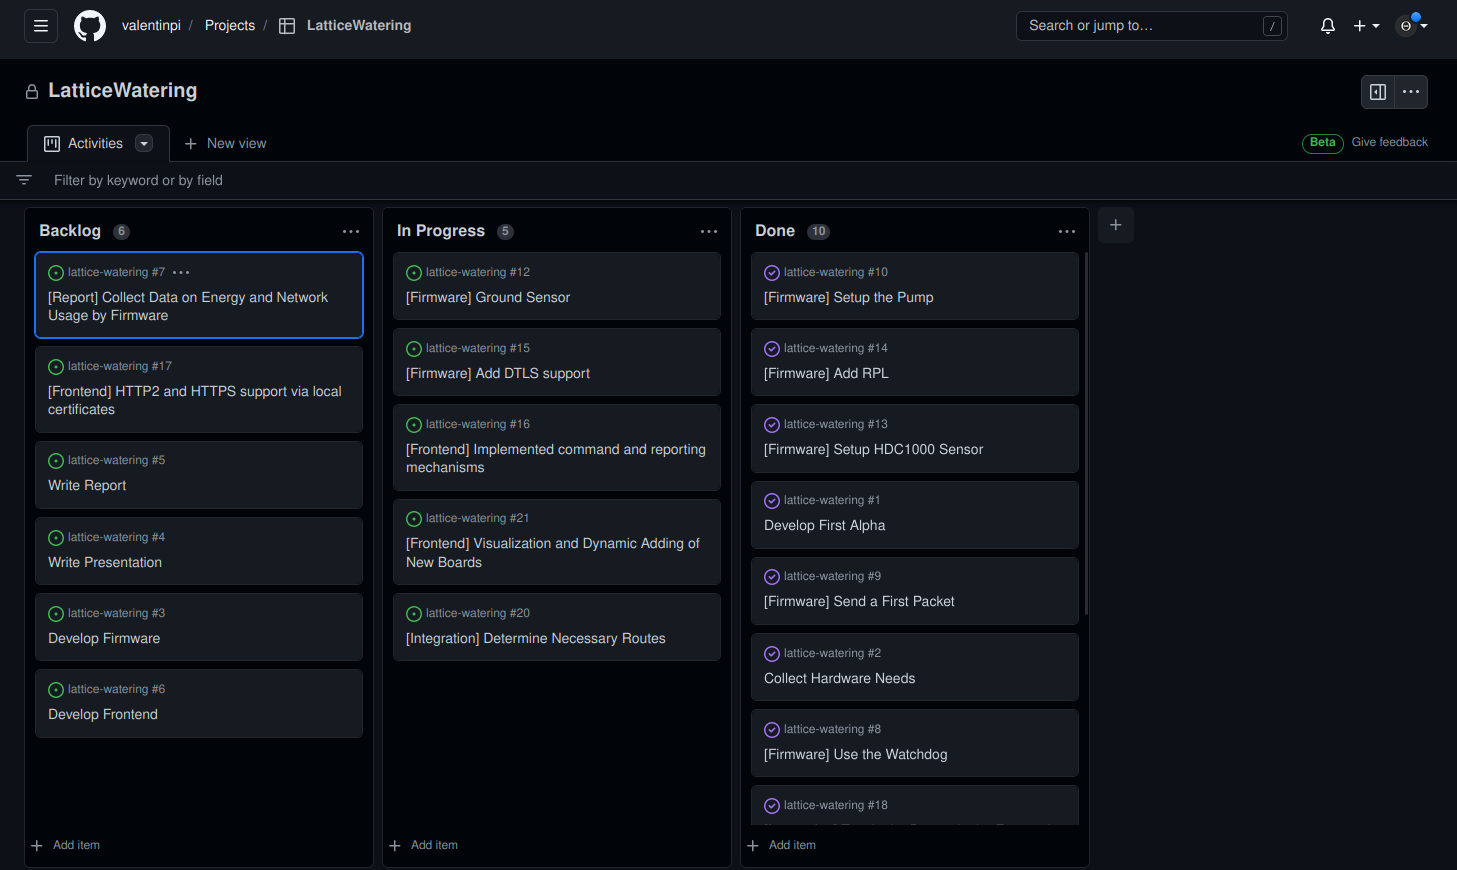
\includegraphics[width=\linewidth]{img/kanban_board.png}
        \Description{Figure of Kanban board we used.}
        \caption{The kanban project board. (State: 13th June, 18:32)}
        \label{fig:kanban_board}
    \end{figure}

    \label{sec:hardware} \section{Hardware}

    One major motivation for us was to work close to hardware. The boards and sensory we used came mostly from suggestions by Hauke Petersen, a scientific coworker in the department and lead developer of RIOT OS. In our network, see \cref{sec:network_structure}, we essentially use three types of devices: A host computer which is quite powerful, a border router that translates traffic of a SixLoWPAN network, that is the name for a set of protocols used in low power radio based communication networks, and so-called nodes. The latter two types of boards use class 2 embedded devices (see RFC 7228) with about 32kB of SRAM memory. A sharp eye may criticize that the border router is also quite a weak board, but during development we tried to mitigate this possible problem by reducing its role in the communication network to a pure routing one. In total, we have the following hardware list:
    \begin{enumerate}
        \item One personal computer with the software set up.
        \item Two SAMR21-XPRO boards, one border router and one node.
        \item Two micro USB cables, optionally a battery connector or powerbank.
        \item One DRV8833 motor driver board.
        \item One electronic pump, see the file mentioned below. It should come with a long tube.
        \item One capacitive moisture sensor, see the file mentioned below.
        \item Nine female jumper cables.
        \item Five male jumper cables.
    \end{enumerate}
    This entire list can be found in \texttt{HWSETUP.md} inside of the repository, with descriptions on how to connect the jumper cables. In the repository, one can also find instructions on how to setup the software. However, we assume that the reader is already familiar with RIOT OS and has the appropriate toolchains and \texttt{udev} rules set up.

    \begin{figure*}[htbp!]
        \centering
        \begin{circuitikz}
            \ctikzset{multipoles/dipchip/width=3}
            \draw (0, 0) node[dipchip, num pins=24, hide numbers, draw only pins={15, 23, 24}, no topmark] (B) {\texttt{SAMR21-XPRO}};
            \draw (B.bpin 24) circle[radius=1.5pt];
            \draw (B.bpin 23) circle[radius=1.5pt];
            \draw (B.bpin 15) circle[radius=1.5pt];
            \node [left] at (B.bpin 24) {\texttt{5V0}};
            \node [left] at (B.bpin 23) {\texttt{GND}};
            \node [left] at (B.bpin 15) {\texttt{PB03}};
            \draw (B.bpin 24) -- +(7, 0) node[above, pos=0.5] {5V};
            \draw ($(B.bpin 24)+(7, 0)$) circle[radius=1.5pt];
            \draw (B.bpin 23) -- +(2, 0);
            \draw ($(B.bpin 24)+(7, -4)$) node[nigfete, bodydiode, tr circle] (mos) {}
                (mos.source) node[anchor=north, below right] {\texttt{S}}
                (mos.gate) node[anchor=east, above left]     {\texttt{G}}
                (mos.drain) node[anchor=south, above right]  {\texttt{D}};
            \draw (mos.source) -- +(0, -2);
            \draw ($(mos.source)+(0, -2)$) -- ($(mos.source)+(-2, -2)$);
            \draw ($(mos.source)+(-2, -2)$) circle[radius=1.5pt];
            \draw (mos.gate) -- +(-1, 0);
            \draw ($(mos.gate)+(-1, 0)$) circle[radius=1.5pt];
            \draw ($(mos.source)+(-2, -2)$) -- ($(mos.source)+(-5, -2)$) -- ($(B.bpin 23)+(2, 0)$);
            \draw ($(mos.gate)+(-3.5, 0)$) to[R=\qty{200}{\ohm}] ($(mos.gate)+(-1, 0)$);
            \draw ($(mos.gate)+(-1, 0)$) to[R=\qty{5}{\kilo\ohm}] ($(mos.source)+(-2, -2)$);
            \draw ($(mos.gate)+(-3.5, 0)$) -- ($(mos.gate)+(-3.5, -0.775)$) -- (B.bpin 15);
            \draw ($(B.bpin 24)+(7, 0)$) -- +(0, -1);
            \draw ($(B.bpin 24)+(7, -1.5)$) circle[radius=0.5];
            \node at ($(B.bpin 24)+(7, -1.5)$) {\texttt{P}};
            \draw ($(B.bpin 24)+(7, -2)$) -- (mos.source);
        \end{circuitikz}
        \Description{Figure of the original circuit idea for the pump.}
        \caption{Original circuit idea for the pump. This is a rough sketch, and does not exactly represent the circuitry involved. \((\texttt{P}, \texttt{S}, \texttt{G}, \texttt{D}) = (\text{Pump}, \text{Source}, \text{Gate}, \text{Drain})\). We credit Hauke Petersen with the design of this circuit.}
        \label{fig:circuit_idea}
    \end{figure*}

    As for the hardware itself, we want to share only one more story during development. There was a very specific problem at the start of the project, which halted development shortly, but we managed to catch up as we were quite early when we tried to obtain hardware. The problem is that connecting the pump to the node boards themselves, the ones of model \texttt{SAMR21-XPRO}, the pump induces a current of 200mA. This is too much for the GPIO pins to handle, as one can read in the manual for the board, which we have provided in the \texttt{man} folder of the repository.

    Together with Hauke, we discussed possible solutions to this problem, of which at first the most promising one can be seen in \cref{fig:circuit_idea}. We can see that in this schematic the pump is connected to the board via the GPIO connection and both the 5 volt and ground pins. We shall not go into the details of the electronics of that circuit and why it would work under ideal conditions. According to Hauke this is rather a matter of experience. What the may note is that the essential idea is that current flows between the \texttt{5V0} and \texttt{GND} pins to drive the pump if and only if as soon as an electric signal on the \texttt{PB03} pin is raised and thus the transistor is switched. We built the circuit, but as it turns out the transistor we had available failed. So Hauke proposed that we obtain some predesigned motor boards, which are documented in \texttt{HWSETUP.md}. Those boards already have this circuit idea embedded in one board, meaning that there are some resistors and a transistor built onto one board and we just have to connecting everything properly.

    \begin{figure}[!hbtp]
        \centering
        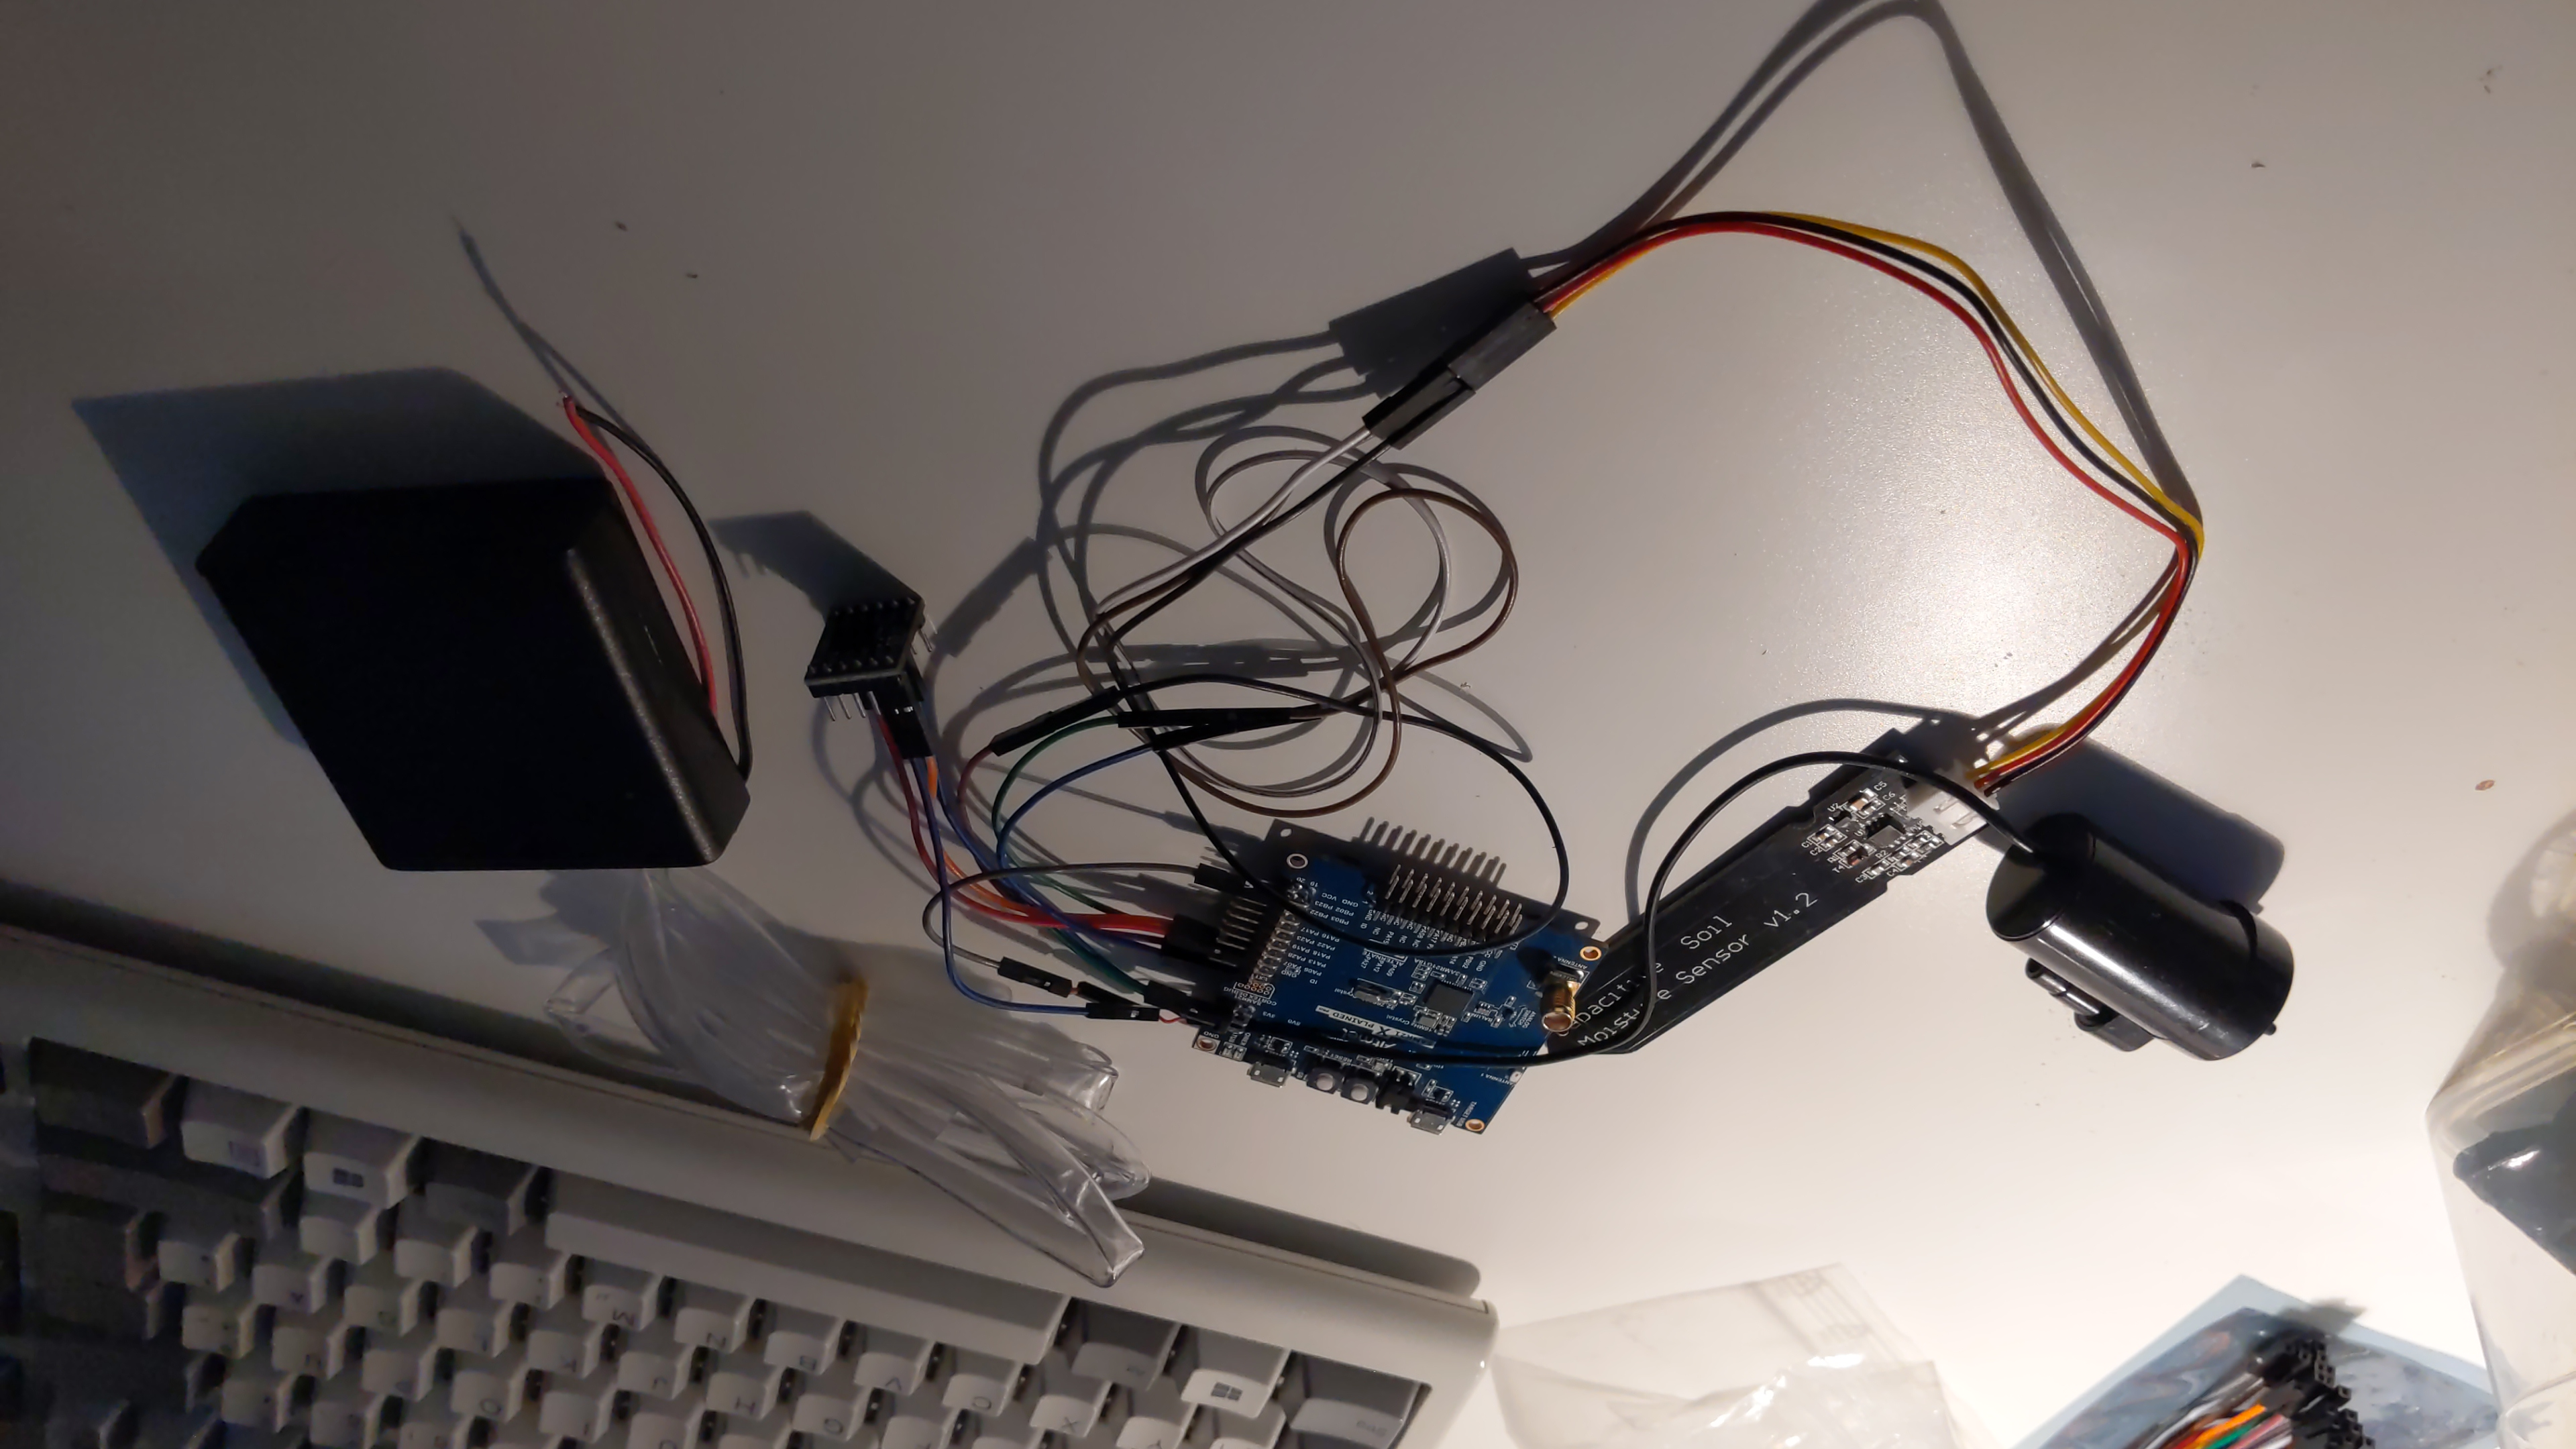
\includegraphics[angle=180, width=\linewidth]{img/almost_fully_connected_node.jpg}
        \Description{Picture of an almost fully connected node.}
        \caption{An almost fully connected node. We can see that it is quite a cable salad, in the final presentation we gave we suggested to put everything in a casing so that it looks more compact. On the right we can see the driver board that connects the pump and the board, and on the left the capacitive moisture sensor that one would put into soil to measure humidity. It is not \emph{fully} connected, because for one we would place t he moisture sensor into soil, the pump into water, whilst connecting it with the plastic tube shown on the right, and then we would connect the board to a power source. This could be a battery connector, here the large case on the right that can hold up to four AA batteries, or a simple micro USB cable.}
        \label{fig:almost_fully_connected_node}
    \end{figure}

    To get a feeling for what an almost fully connected node looks like, one may refer to \cref{fig:almost_fully_connected_node}.

    \label{sec:network_structure} \section{Network Structure}

    The structure of our network is illustrated in \cref{fig:network_structure}. In \cref{sec:hardware}, we described that for our devices we had a host, a border router and nodes. We want to precise that a bit.

    The network is divided into two parts. There is the connection between the border router and the host. It is a USB connection in our case, but it uses a technology called \texttt{ethos}, which is a small module/program that RIOT OS developed for setting up Ethernet networks based on serial connections. The user operating the host starts the \texttt{ethos} program on a serial port with the border router and that program sets up a layer 2 connection with the board by binding the port and transfering data inbetween. The physical layer connection is provided by the USB connection. At the same time, the USB port provides the border router with power, so we do not need to connect it to a battery or a plug seperately.

    We have wrapped the \texttt{ethos} program inside of a small \texttt{Makefile} command, which one can inspect in \texttt{br/Makefile}. Besides starting the program, the command also creates a virtual network tap device, which is only natively possible on Linux at this moment. The virtual network device is bounded by \texttt{ethos} and gets assigned the IP \texttt{fc00::}, which is an IPv6 \emph{Unique Local Address} (ULA). With that, we follow the recommended conventions for unique local addresses described in RFC 4193. The border router assigns itself the fixed address \texttt{fc00::1}, such that we may easily debug network issues. So the network prefix \texttt{fc00::/64} at this moment is made up of two devices.

    We introduce the second network. The nodes are designed to be low power devices that can be scattered around a small area such as a small house. They connect themselves to the fixed IP address \texttt{fc00:0:0:1::}, which is the address that we assign the IEEE802154 network interface of our border router. Note that it has such a radio interface for receiving IP packets from the nodes and forwarding them to the frontend. The addresses of the nodes are made up of the prefix \texttt{fc00:0:0:1::/64} and the last 64 bits replaced with the MAC address of the node. So these IP addresses are predetermined. The professor already suggested using an application specific specifier, so this could be an improvement over this rather rough way of designing the layer 3 addressing.

    So we have now described how the devices are setup. But we want to shine a bit more light on the other protocols that are involved in the network. For layer 3, we only use \emph{IPv6} as it is the more modern standard and since RIOT does not support IPv4. We also learned that IPv6 replaces some old technologies such as ARP with new ones such as its very own Neighbor Discovery routines and general layer 2 address resolution techniques.
    
    To perform routing inside of the lossy IoT network, we use the \texttt{Routing Protocol for Low-Power and Lossy Networks} (RPL). RFC 6550 describes it. The short idea is that we may create routing topologies for far areas by designating some network entities as roots such that the nodes can build up graph theoretic tree structures, which are just \emph{Directed Acylic Graphs} (DAGs). The routing now happens in the way that a node has exactly one entity it can route a packet to. Note that the RFC also suggests some useful topologies for these routing schemes, such as a \emph{Destination-Oriented DAG} (DODAG), where there is only one root. This is useful in our case, as it simplifies the routing by quite a lot.

    These three technologies presented two extremes for us during development. For one, setting up \texttt{ethos} and the border router routing table, to route between the IEEE802154 and Ethernet interfaces, yielded unneeded error searches while we were trying to apply the knowledge from the tutorials that were given on the RIOT OS page. The most usual error was that packets just were not routed between the nodes and the host. We checked that by using the ICMP modules from RIOT from shell and sending pings between our fixed IP addresses, see above. Using a snooping tool such as \emph{Wireshark} on the host, we also checked the traffic in hopes of finding out our issues. We cannot replicate all that went wrong during this phase. The professor suggested that we should make proposals on how to improve the RIOT tutorials, but due to stress we have not yet done so. Perhaps the underlying issue also was that the team was just not familiar enough with RIOT and the protocols involved. That is the first extreme: Huge difficulties whilst setting up \texttt{ethos} and IPv6 routing. The second extreme was the very pleasant experience in setting up RPL, which just consisted of designating the border router as a DAG root and then just loading the appropriate modules into both \texttt{br} and \texttt{fw}.

    \begin{figure*}[!hbtp]
        \centering
        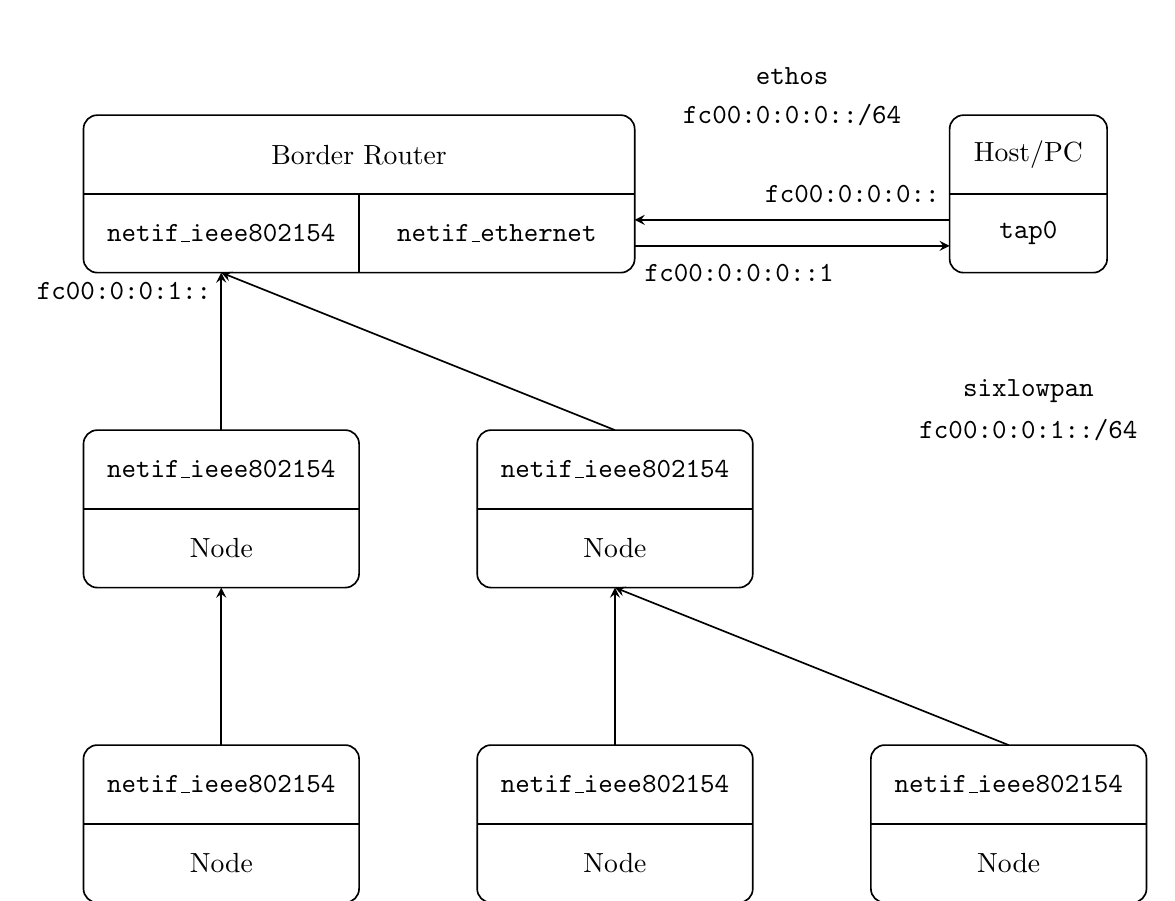
\begin{tikzpicture}[>=stealth, semithick]
            \draw[rounded corners=5pt] (-1, -1) rectangle (1, 1);
            \draw[draw=none] (-1, 0) -- (1, 1) node[pos=0.5] {Host/PC};
            \draw (-1, 0) -- (1, 0);
            \draw[draw=none] (-1, 0) -- (1, -1) node[pos=0.5] {\texttt{tap0}};

            \draw[rounded corners=5pt] (-12, -1) rectangle (-5, 1);
            \draw[draw=none] (-12, 0) -- (-5, 1) node[pos=0.5] {Border Router};
            \draw (-12, 0) -- (-5, 0);
            \draw (-8.5, 0) -- (-8.5, -1);
            \draw[draw=none] (-12, 0) -- (-8.5, -1) node[pos=0.5] {\texttt{netif\_ieee802154}};
            \draw[draw=none] (-8.5, 0) -- (-5, -1) node[pos=0.5] {\texttt{netif\_ethernet}};
            \draw[->] (-1, -0.33) -- (-5, -0.33);
            \node[left] at (-1, 0) {\texttt{fc00:0:0:0::}};
            \node[right] at (-5, -1) {\texttt{fc00:0:0:0::1}};
            \node at (-3, 1.5) {\texttt{ethos}};
            \node at (-3, 1) {\texttt{fc00:0:0:0::/64}};
            \draw[->] (-5, -0.66) -- (-1, -0.66);
            \node[below left] at (-12+1.75, -1) {\texttt{fc00:0:0:1::}};

            \newcommand{\networknode}[2]{
                \draw[rounded corners=5pt] (#1, #2) rectangle (#1+3.5, #2-2);
                \draw (#1, #2-1) -- (#1+3.5, #2-1);
                \draw[draw=none] (#1, #2) -- (#1+3.5, #2-1) node[pos=0.5] {\texttt{netif\_ieee802154}};
                \draw[draw=none] (#1, #2-1) -- (#1+3.5, #2-2) node[pos=0.5] {Node};
            }

            \networknode{-12}{-3};
            \networknode{-7}{-3};
            \networknode{-12}{-7};
            \networknode{-7}{-7};
            \networknode{-2}{-7};

            \draw[->] (-12+1.75, -3) -- (-12+1.75, -1);
            \draw[->] (-7+1.75, -3) -- (-12+1.75, -1);
            \draw[->] (-12+1.75, -7) -- (-12+1.75, -5);
            \draw[->] (-7+1.75, -7) -- (-7+1.75, -5);
            \draw[->] (-2+1.75, -7) -- (-7+1.75, -5);

            \node at (0, -2.5) {\texttt{sixlowpan}};
            \node at (0, -3) {\texttt{fc00:0:0:1::/64}};
        \end{tikzpicture}
        \Description{Figure of the network topology. We can see that the border router acts between the host and the SixLoWPAN network.}
        \caption{The Network Topology. The device interfaces are named after our code. The \texttt{tap0} device is named after the typical Linux entry. The network stack is based on COAP, DTLS, UDP, 6LoWPAN IPHC and FRAG, RPL, IPv6. The global IP addresses of the nodes inside the \texttt{fc00:0:0:0:0:0:0:1::/64} network are chosen by appending the Layer 2 addresses to the network prefix. The DAG structure of the RPL network is shown schematically.}
        \label{fig:network_structure}
    \end{figure*}

    As for the other protocols used, our communication principle was to design it as energy efficient and with as small and as few regularly sent packets as possible. Thus we ruled out any form of state based communication besides DTLS as we cannot compromise on security: For one, an attacker might be interested in damaging expensive plants to hurt the owner financially and emotionally. Our threat model assumes that no node is compromised, which is why we used Pre-Shared Keys, see \cref{subsec:dtls} for more details.

    So in the standard ISO/OSI model we skip layers five and six, besides what protocol management introduces in form of certain saved cookies by the DTLS protocol, and turn to layers four and seven. The former is not very interesting: We just use UDP. For all communication between the nodes and the host, we use non-confirmable CoAP packets. The exact methods between that can be called using CoAP on the node or on the host are described in the file \texttt{METHODS.md}. Note that since each node uses DTLS with the host, meaning that they both share a secure session, these RPC calls are all secured and unique to one communication. More precisely, in RIOT we use the abstraction GCoAP or GCoAP-DTLS, which allows us to define method listeners directly and send out packages quite easily, whilst possibly introducing a slight bit more of packet duplication, as we do not directly use RIOT OS Packet Buffers.

    \section{Application Structure}

    \begin{figure*}[!hbtp]
        \centering
        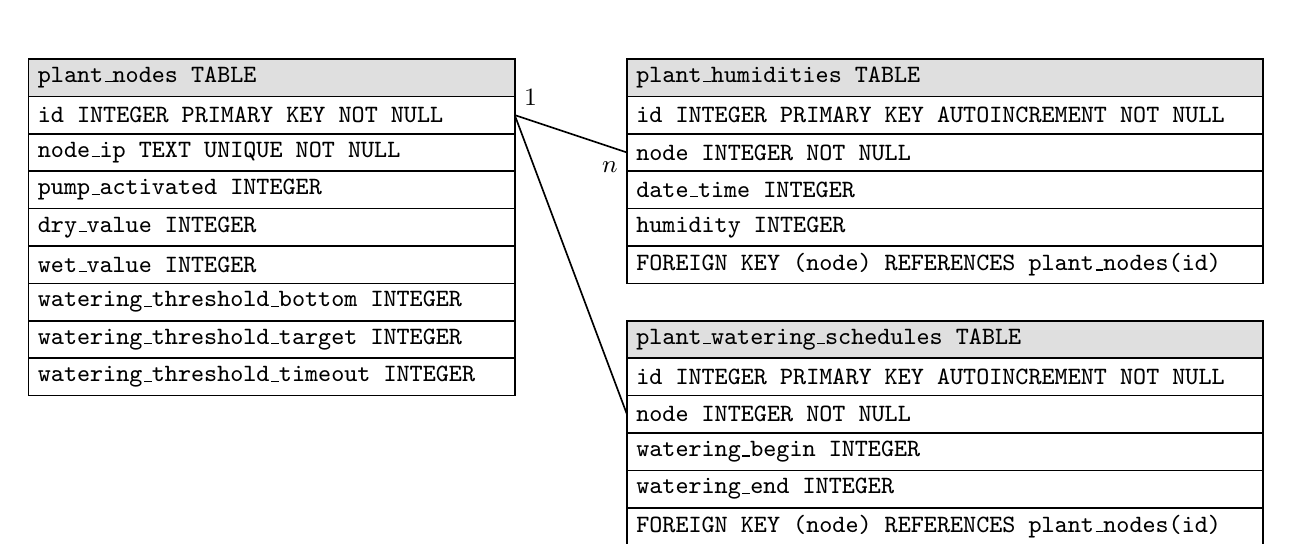
\begin{tikzpicture}[>=stealth, semithick, scale=0.95]
            \small
            \newcommand{\column}[3]{
                \draw[#1] (0, #3) rectangle (6.5, #3-0.5);
                \node[right] at (0, #3-0.25) {#2};
            }
            \column{fill=gray!25}{\textbf{\texttt{plant\_nodes TABLE}}}{0};
            \column{}{\texttt{id INTEGER PRIMARY KEY NOT NULL}}{-0.5};
            \column{}{\texttt{node\_ip TEXT UNIQUE NOT NULL}}{-1};
            \column{}{\texttt{pump\_activated INTEGER}}{-1.5};
            \column{}{\texttt{dry\_value INTEGER}}{-2};
            \column{}{\texttt{wet\_value INTEGER}}{-2.5};
            \column{}{\texttt{watering\_threshold\_bottom INTEGER}}{-3};
            \column{}{\texttt{watering\_threshold\_target INTEGER}}{-3.5};
            \column{}{\texttt{watering\_threshold\_timeout INTEGER}}{-4};
            \renewcommand{\column}[3]{
                \draw[#1] (8, #3) rectangle (16.5, #3-0.5);
                \node[right] at (8, #3-0.25) {#2};
            }
            \column{fill=gray!25}{\textbf{\texttt{plant\_humidities TABLE}}}{0};
            \column{}{\texttt{id INTEGER PRIMARY KEY AUTOINCREMENT NOT NULL}}{-0.5};
            \column{}{\texttt{node INTEGER NOT NULL}}{-1};
            \column{}{\texttt{date\_time INTEGER}}{-1.5};
            \column{}{\texttt{humidity INTEGER}}{-2};
            \column{}{\texttt{FOREIGN KEY (node) REFERENCES plant\_nodes(id)}}{-2.5};
            \renewcommand{\column}[3]{
                \draw[#1] (8, #3-3.5) rectangle (16.5, #3-4);
                \node[right] at (8, #3-3.75) {#2};
            }
            \column{fill=gray!25}{\textbf{\texttt{plant\_watering\_schedules TABLE}}}{0};
            \column{}{\texttt{id INTEGER PRIMARY KEY AUTOINCREMENT NOT NULL}}{-0.5};
            \column{}{\texttt{node INTEGER NOT NULL}}{-1};
            \column{}{\texttt{watering\_begin INTEGER}}{-1.5};
            \column{}{\texttt{watering\_end INTEGER}}{-2};
            \column{}{\texttt{FOREIGN KEY (node) REFERENCES plant\_nodes(id)}}{-2.5};
            \draw (6.5, -0.75) -- (8, -1.25);
            \draw (6.5, -0.75) -- (8, -4.75);
            \node[above right] at (6.5, -0.75) {1};
            \node[below left] at (8, -1.25) {\(n\)};
        \end{tikzpicture}
        \Description{Figure of our database schema. It shows all three tables. - One for storing general node information, one for humiditiy values and one for the watering schedules.}
        \caption{The SQLite database schema. The upper left table persists some of the current configurations and the current status for each node. The network structure guarantees the uniqueness of the IPs, so it suffices to use them as an identifier in our use case. One may consider replacing this with an application-specific ID as we have described above, which may for one have to persist on the nodes themselves, e.g. via EEPROM. One can find this exact structure in \texttt{front/db.js}. The other two tables store the humidity values over time of the plants such that we can access them later on, and the current fixed-time watering schedules. Remember that we offer threshold-based and schedule-based watering.}
        \label{fig:db_scheme}
    \end{figure*}

    In total, we have developed \emph{five} different applications which all work together.
    \begin{itemize}
        \item \texttt{fw}: The firmware that is deployed on the nodes themselves reads out sensor values and sends them the host.
        \item \texttt{br}: The border router acts as a mediator between the lossy SixLoWPAN and the local Ethos network with the host. It allows the nodes that are reachable to send messages to the host computer.
        \item \texttt{proxy}: The proxy receives DTLS traffic from the nodes, decrypts them, appends a target IP and forwards them to the backend software written in Node.JS.
        \item \texttt{front}: The backend software serves the webpage for the frontend and manages the database.
        \item \texttt{www}: The website written in JavaScript, which may or may not be considered a seperate application, offers the user
    \end{itemize}

    The frontend also stores the humidity data and the current status of nodes according to the data regularly transmitted on the \texttt{/data} route. \cref{fig:db_scheme} shows the database scheme. We use SQLite, a very small and fast single user database, which suffices for our usecase. For something larger we may need multiple users and thus a different database, which should not be too difficult given the complexity of our current database operations.

    \label{subsec:dtls} \subsection{DTLS}

    The \texttt{Datagram Transport Layer Security} protocol aims to introduce security of communication to the unsecured UDP protocol. DTLS (RFC 4347) behaves similiar to TLS in that before a communication may take place, a participant first has to negotiate secure ciphers for communication, but not in that the packets are assured to arrive in the correct order or fully. However, the protocol guarantees this for the transmitted payload data.

    To enable DTLS for our application, we had to first include the \texttt{gcoap\_dtls} package in our \texttt{fw} in RIOT with a \emph{Pseudo Random Number Generator} (PRNG) and an appropriate library, in our case \texttt{tinydtls}. We did not use WolfSSL as it is currently not supported by the \texttt{gcoap} RIOT abstraction for CoAP.
    
    Sadly introducing DTLS to our communication turned out to give us some of the worst trouble we had in the project, because Node.JS support for DTLS is in quite a rough state as this time, as none of the libraries we were trying out worked with. Note that there is an official issue for introducing DTLS to Node, but the developers there are not very active at the moment: \cite{node-dtls-issue}. And it is not clear if this will be resolved anytime soon, as the new protocol QUIC emerged. To be precise, we tried the following libraries:

    \begin{itemize}
        \item \texttt{dtls} \cite{npm-dtls}: This NPM package just does not contain anything. 
        \item \texttt{openssl-dtls} \cite{npm-openssl-dtls}: Node FFI bindings that work, but during development, OpenSSL did not work with the ciphersuite \texttt{TLS\_PSK\_WITH\_AES\_128\_CCM\_8}, which is used by \texttt{tinydtls}. The cipher negotiation fails for to us unknown reasons.
        \item \texttt{node-mbed-dtls} \cite{npm-node-mbed-dtls}: Based on \texttt{mbed-dtls}, but with the same issue as with \texttt{openssl-dtls}.
        \item \texttt{werift-dtls} \cite{npm-werift-dtls}: Crashes upon receival of a Client Hello packet, also very poorly documented code. As it seems, it is part of a bigger set of tools for WebRTC.
        \item \texttt{nodejs-dtls} \cite{npm-nodejs-dtls}: Only contains a DTLS client.
        \item \texttt{@nodertc/dtls} \cite{npm-nodertc-dtls}: Only contains a DTLS client. Development for a server seems to be ongoing on the \texttt{main} branch on GitHub, but with no recent activity
        \item \texttt{node-dtls-proxy} \cite{npm-node-dtls-proxy}: Crashes upon receival of a Client Hello packet.
        \item \texttt{goldy} \cite{github-goldy}: Cipher negotiation with a node fails, also it seems that the proxy only forwards traffic between two peers, but we want to be dynamic in that multiple nodes can connect to the server and we do not need to start a proxy for each one seperately.
    \end{itemize}

    There was also a short unsuccessful attempt at writing a very small proxy using python-dtls, but this was conceptually flawed, as the proxy needs to know where to route the packets from the frontend. In the end, as the board uses \texttt{tinydtls}, we decided to use Rust to write a small proxy using \texttt{tinydtls-sys}. \cref{fig:dtls_proxy} shows the structure of the proxy, which acts in the middle of the communication between the frontend and the nodes. Note that the proxy is running on the host computer.

    \begin{figure}[!hbtp]
        \centering
        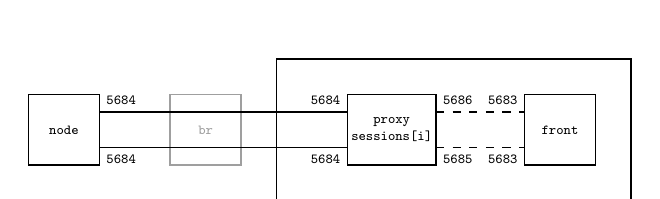
\begin{tikzpicture}[>=stealth, semithick, scale=0.45]
            \tiny
            \draw (0, 0) rectangle (2, -2) node[pos=0.5] {\texttt{node}};
            \draw[draw=gray!75] (4, 0) rectangle (4+2, -2) node[pos=0.5] {\textcolor{gray!75}{\texttt{br}}};
            \draw (7, 1) rectangle (8+9, -3) node[pos=0.5] {};
            \draw (9, 0) rectangle (9+2.5, -2) node[align=center, pos=0.5, text width=2cm] {
                \texttt{proxy}\\
                \texttt{sessions[i]}
            };
            \draw (14, 0) rectangle (14+2, -2) node[pos=0.5] {\texttt{front}};
            \draw (2, -0.5) -- (9, -0.5);
            \node[above right] at (2, -0.5) {\texttt{5684}};
            \node[above left] at (9, -0.5) {\texttt{5684}};
            \draw (2, -1.5) -- (9, -1.5);
            \node[below right] at (2, -1.5) {\texttt{5684}};
            \node[below left] at (9, -1.5) {\texttt{5684}};
            \node[above right] at (11.5, -0.5) {\texttt{5686}};
            \node[below right] at (11.5, -1.5) {\texttt{5685}};
            \node[above left] at (14, -0.5) {\texttt{5683}};
            \node[below left] at (14, -1.5) {\texttt{5683}};
            \draw[dashed] (11.5, -0.5) -- (14, -0.5);
            \draw[dashed] (11.5, -1.5) -- (14, -1.5);
        \end{tikzpicture}
        \Description{Figure of the DTLS proxy. It shows how the proxy takes DTLS traffic from nodes, translates them to general CoAP and forwards them to the host.}
        \caption{The DTLS proxy. Secure channels are represented by thick lines, insecure channels by thin lines. We have denoted the UDP ports. The \texttt{br} is greyed out as it only routes the packets. Note that each node has its own DTLS session registered in the proxy, the index \texttt{i} is for illustration. There can be at most 16 as of writing. Also the \texttt{proxy} has two sockets for communication with the backend, simply due to constraints with the C FFI in Rust which we were not able to fix by this time.}
        \label{fig:dtls_proxy}
    \end{figure}

    When a board wants to send data through the \texttt{/data} CoAP POST method of the host, it first tries to establish a secure DTLS session. For that, it sends a Client Hello packet and then does cipher negotation such that the future communication partners know how to encrypt and decrypt packages. One special property of our communication is that we use \emph{Pre-Shared Keys} (PSKs). Via an \emph{identity message}, the server tells the node which pre-shared key to use. We only have one, so we called our identity \texttt{default}. The PSKs themselves are just random data, here 16 bytes, as RIOT does not support longer keys. We automatically generate them using a script, and recommend that inside of \texttt{README.md}.

    \bibliographystyle{unsrt}
    \section{Evaluation Closing Words}

    \bibliography{report}

    %\listoffigures
\end{document}
